\documentclass[5p]{elsarticle}

\usepackage{lineno,hyperref}
\modulolinenumbers[100]

% to be able to introduce several figures that occupy the width of the two columns.
\usepackage{subfigure}

% for merge cells
\usepackage{booktabs}
\usepackage{bookmark}

% for newline in a table cell
\usepackage{makecell}

% for table border lines and padding
\setlength{\heavyrulewidth}{1.5pt}
\setlength{\abovetopsep}{4pt}

\journal{International Journal for Medical Informatics}

%%%%%%%%%%%%%%%%%%%%%%%
%% Elsevier bibliography styles
%%%%%%%%%%%%%%%%%%%%%%%
%% To change the style, put a % in front of the second line of the current style and
%% remove the % from the second line of the style you would like to use.
%%%%%%%%%%%%%%%%%%%%%%%

%% Numbered
%\bibliographystyle{model1-num-names}

%% Numbered without titles
%\bibliographystyle{model1a-num-names}

%% Harvard
%\bibliographystyle{model2-names.bst}\biboptions{authoryear}

%% Vancouver numbered
%\usepackage{numcompress}\bibliographystyle{model3-num-names}

%% Vancouver name/year
%\usepackage{numcompress}\bibliographystyle{model4-names}\biboptions{authoryear}

%% APA style
%\bibliographystyle{model5-names}\biboptions{authoryear}

%% AMA style
%\usepackage{numcompress}\bibliographystyle{model6-num-names}

%% `Elsevier LaTeX' style
\bibliographystyle{elsarticle-num}
%%%%%%%%%%%%%%%%%%%%%%%

\begin{document}

\begin{frontmatter}

\title{Biobank registry implementation: An evaluation of NoSQL databases \\for Philippine Cancer-Phenome Biobanking System}
%% \tnotetext[mytitlenote]{Fully documented templates are available in the elsarticle package on \href{http://www.ctan.org/tex-archive/macros/latex/contrib/elsarticle}{CTAN}.}

%% Group authors per affiliation:
%% \author{Elsevier\fnref{myfootnote}}
%% \address{Radarweg 29, Amsterdam}
%% \fntext[myfootnote]{Since 1880.}

%% or include affiliations in footnotes:
\author[miuaddress]{Philip John C. Sales}\corref{mycorrespondingauthor}
\ead{pcsales@up.edu.ph}

% \author[regenlabaddress]{Michael C. Velarde\corref{mycorrespondingauthor}}
\author[regenlabaddress]{Michael C. Velarde\fnref{regenwebsite}}
\ead{mcvelarde@up.edu.ph}

\author[miuaddress,casaddress]{Ariel S. Betan}
\ead{asbetan@up.edu.ph}

%% \ead[url]{https://regenlab.weebly.com}

\author[miuaddress]{Alvin B. Marcelo}
%% \cortext[mycorrespondingauthor]{Corresponding author}
\ead{admarcelo@up.edu.ph}

\cortext[mycorrespondingauthor]{Corresponding author at Medical Informatics Unit,  UP College of Medicine, Tel. +63(2) 536 1396} 
\fntext[regenwebsite]{https://regenlab.weebly.com}

\address[miuaddress]{Medical Informatics Unit, College of Medicine, University of the Philippines, Ermita, Metro Manila}
\address[regenlabaddress]{Regenerative Biology Research Laboratory, Institute of Biology, University of the Philippines, Quezon City, Diliman }
\address[casaddress]{College of Arts and Sciences, Department of Social Sciences, University of the Philippines, Ermita, Metro Manila}

\begin{abstract}

\paragraph{Background and objective:} The field of healthcare is rapidly accumulating data of complex types and formats. 
The current methods of storing data relies heavily on traditional relational database management system (RDBMS) which have notable limitations 
in managing clinical and biomedical data. Thus, a constant demand for alternative approach is in place. 
Among the available solutions, NoSQL databases had been cited as a viable option due to its numerous advantages in handling healthcare data challenges. 

\paragraph{Methods:} This study evaluated different types of NoSQL databases using an database evaluation framework tailored for healthcare context.

\paragraph{Results:} The application-specific evaluation criteria showed that document-based type is the best choice for extensibility, flexibility, and query 
readability whereas key-value pair is the most efficient in performance and scalability. Moreover, columnar-wide has the edge in 
storage capacity. 

\paragraph{Conclusion:} Among the shortlisted databases, MongoDB - a document type NoSQL was found to be the recommended choice for the current implementation 
and immediate need of the biobank information system.

\end{abstract}

\begin{keyword}
\texttt Clinical data\sep relational database\sep NoSQL\sep biobanking
\sep database evaluation framework\sep health information system
\end{keyword}

\end{frontmatter}

\linenumbers

\section{Introduction}
The increasing size and complexity of data being generated in healthcare industry is reaching
 to the point of being unmanageable \cite{R.Kumar2015208,M.Ercan190510}. This was brought about 
 by the technological advances in medical and biomedical fields which have highlighted the importance 
 of collecting and storing data to benefit clinical research and medical services.

Currently, storage of clinical data largely relies on relational database management systems 
\cite{Z.Goli-Malekabadi201675,K.Lee201299} and has been the most common approach of data 
storage since the 90’s \cite{P.Atzeni1993}. From the time of its origins in the 1970’s, the relational 
model had been adapted widely in many database management systems \cite{K.Berg201329,D.Suciu200139} and 
had remained unchanged for decades \cite{M.Ercan190510}. This modeling approach had become the de 
facto standard for most industries, but remains ineffective in the field of healthcare due to the characteristics
of clinical and biomedical data.

Healthcare data are dynamic, hierarchal, sporadic, and heterogeneous in nature. 
It is stored in various types including free text, coded data elements, images, signals, logs, or notes that is formatted in either structured, semi-structured, 
or unstructured presentation \cite{M.Ercan190510,K.Lee201299,C.S.Kruse201638,S.White201413,S.Wasan1192016}.
The heterogeneity of formats, high volume exchange, and dynamic structure makes it difficult to model and manage health 
data using the traditional relational database \cite{K.Lee201299,H.Al-Fatlawi2015122,O.Schmitt20121,Y.Jin2011288}.

In addition, one of the major drawback of relational database is the need for pre-designed schema. 
Predefining the data structure is impractical since pre-determing the combination and variety of data fields to be collected in a medical record is unrealistic \cite{K.Lee201299}. 
%The issue of pre-defining data structure is the fact that it is unrealistic to pre-determine all the variety of data fields to be collected in a medical form much less a clinical record \cite{K.Lee201299}. 

Succintly, RDBMS is not flexible, scalable, and extensible to overcome the problem of constantly changing requirements, various formats, increasing volume, and the continuous need for updates in healthcare data \cite{Z.Goli-Malekabadi201675,K.Lee201299,H.Al-Fatlawi2015122,O.Schmitt20121,Y.Jin2011288}.

Against these backdrops, there is a constant demand and practical need for alternatives outside the conventional relational data modeling approach. 
As evidence there are increasing researches and industry projects on databases that are driven by the practical experience of the conflicting static 
nature of relational database and dynamic characteristics of healthcare data \cite{M.Ercan190510}.

Out of the wide spectrum of viable alternatives, this study identified NoSQL database as supported by literature to be suitable in addressing the challenges of 
healthcare data. NoSQL approach had attracted the attention of non-clinical industries \cite{C.S.Kruse201638,Z.Parker20131,G.D.Ferreira2013125} and researchers 
due to its flexibility, scalability, velocity, and availability which addresses the limitations of relational databases \cite{M.Ercan190510}. 
While there are significant advantages of using NoSQL database, there is limited research which has evaluated the use of NoSQL databases in the healthcare domain.

Additionally, it is not always straightforward to declare which database type is better than the other. Concerns are raised in selecting which among the list of 225 NoSQL databases \cite{S.Edlich2018} 
can best address the healthcare data challenge. To date, there is a paucity of literature that provides guiding principle, standard protocol, or framework on how to
evaluate of database for healthcare industry.

In light of the foregoing, this study attempted to evaluate three NoSQL database types (i.e. document based, columnar wide, key-value pair) using an systematic evaluation approach. 

The sections below are organized as follows.
Section 2 offers an overview on research project context and the evaluation approach taken. 
Section 3 describes the methodology performed for the testing and prototyping of each NoSQL database type.
The final results of the application-specific evaluation criteria are discussed in section 4. 
Subsequently, a conclusion is given in section 5.

\section{Background}
\subsection{Project Context}
Establishing that relational database have notable limitations in managing the nature of healthcare data \cite{Z.Goli-Malekabadi201675,K.Lee201299,H.Al-Fatlawi2015122,O.Schmitt20121,Y.Jin2011288} is one thing. 
Proposing an alternative solution that undergoes a systematic way of evaluation is another. The latter is the undertaking that this paper aimed to implement.

In relation to Philippine scenario, one of the initiative of Philippine-California Advanced Research Institutes (PCARI) Project is to implement 
of Philippine Cancer Phenome-Biobanking System. The development of this pilot project will serve as a model HIS with optimism 
of going national scale. The data challenges mentioned are applicable to the context of the biobank information system. 
Critical to the success of the system is the appropriate evaluation and selection of data modelling approach and database technology.


Technology selection or evaluation framework are constructs predominantly used in the field of business sectors with focus only upon management and financial 
decisions \cite{C.Chan2010300}, but dearth of source exists when discussing technology or database evaluation for healthcare sector. Moreover, most selection 
practices and evaluation models in digital health technologies are informed by traditional means: word of mouth, internet search, consultant’s advice, expert’s opinion \cite{A.Ostrovsky20141}, 
emerging systems, and technology trend. There are limited models, empirical evidences, and guidelines that facilitate methodological evaluation of database for HIS. 

Thus, this paper adapted a database evaluation framework that will evaluate NoSQL databases against context-based parameters. 

\subsection{Evaluation Approach}
The principles of of this study's evaluation framework is inspired from themes of Digital Selection Framework \cite{A.Ostrovsky20141} 
and the context-driven component evaluation process of Technology Selection Framework for Health Interventions \cite{C.Chan2010300}. 
The aim is to provide reproducible and reusable process in evaluating database that can address application-specific healthcare data requirements.
The main steps are illustrated in Figure \ref{fig.framework} and outlined below. 

\begin{figure*}[ht]
    \centering
    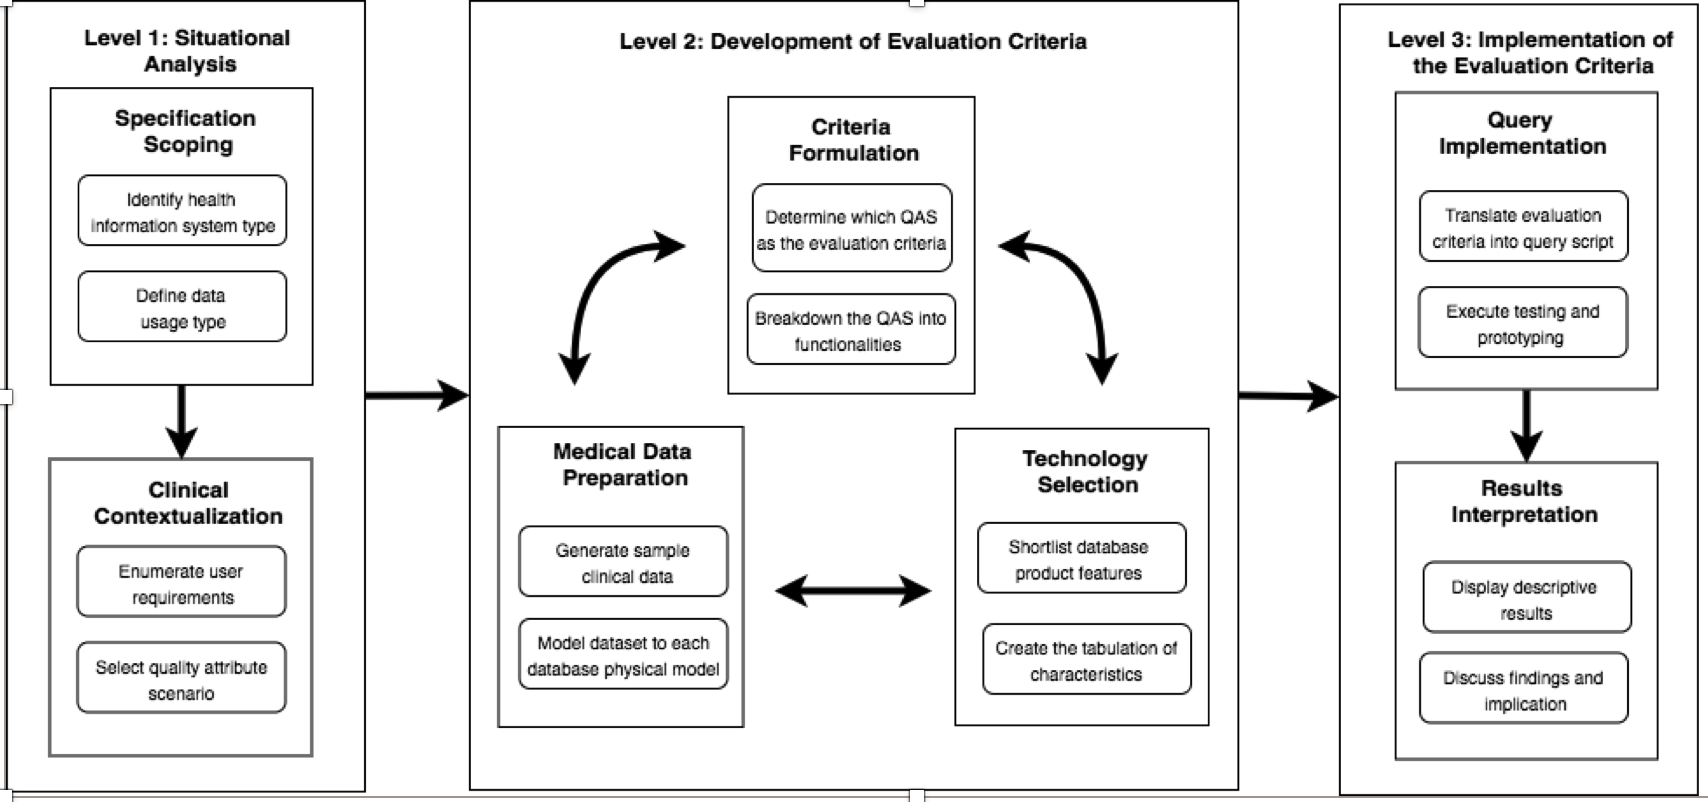
\includegraphics[scale=0.27] {figure}
    \caption{Database Evaluation for Healthcare}\label{fig.framework}
\end{figure*}

\begin{enumerate}
\item \emph{Identifying the scope of the HIS}. In the context of the aforementioned project, this study evaluated the database of choice for a biological specimen inventory and clinical registry type of health information system. The nature of the required system is not transaction intensive but rather storage and reporting exhaustive. With these considerations, the study anticipated the need for a database that can handle voluminous and aggregatable data.
\item \emph{Gathering requirements from stakeholders.} Multiple sessions of focus group discussions and key informant interviews were done as method of elicitation for the quality attribute scenarios, use cases, and business requirements. 
Information gathered served as the basis for the the development of the evaluation criteria. 
This method of consulting the health and allied professionals prioritizes clinical centered need over technology oriented solution.
\item \emph{Formulating the evaluation criteria.} The consolidated and prioritized criteria elicited from the qualitative approach was used as the basis on how the execution of tests was performed. Thus, the findings of this research was context based and can be qualified as a case study. Moreover, the methods applied are generalizable to other HIS database evaluation.
\item \emph{Shortlisting database technology.} On the grounds that the nature of clinical data is highly evolving and dynamic, one of the immediate selection filters is the capability to adapt to schema changes. In consequence, schema-less modelling approach was the logical option; hence, focus on NoSQL was the scope of the implementation. 
This study evaluated only the highly represented and most popular database for each type of the NoSQL category \cite{DBEnginesRanking2018}.
The selected NoSQL databases are MongoDB for the document category, Cassandra for the columnar, and Redis for the key-value.
This paper presented the three different NoSQL types: document based
\item \emph{Model mapping of datasets.} 
Adhering to a clinical information modeling standard enforces the data to be formatted in a semi-structured or structured form making it computable processable searchable, and processable (Weglarz, 2004).

Each database technology has corresponding physical data model and underlying technical requirements that need to be configured prior to the actual loading of the datasets. In using the FHIR standard, schema mapping of the clinical dataset into the physical data storage of each database was implemented.
\item \emph{Executing test scripts against evaluation criteria.} The test scripts were fundamentally derived from the evaluation criteria. Each script was executed multiple times against different workloads on several dataset sizes in different testing configurations to allow rigorous comparison amongst each selected database.
\item \emph{Provide summary of reports and insights.} Summary of results were shown on each enumerated evaluation criteria.
\end{enumerate}

\section{Method}

\subsection{Application-Specific Criteria}
At the end of stakeholders’ group discussions, it was reviewed and found that there were 14 scenarios critical for the biobank system. These scenarios were enumerated then refined into a more verbose description following the QAS template format. Using the identified QAS, further verification with the product champions resulted in a list of 67 functionalities that covers the system’s core features. These functionalities where then grouped into criteria (as seen in table below) and tagged if the functionality is relevant to database operations. The list below is composed of nine (9) criteria that were initially formulated, of which four were excluded as these were not directly related to data storage, with the exception to redundancy criterion. The omission of redundancy was made on the basis of the project scope that is within the researcher’s capacity to implement in the given timeline of the research. Additionally, the last criteria (i.e. query readability) was included as advised by the research panel members.

\subsection{Clinical data using HL7-FHIR}
Having clinical dataset formatted in standard medical information modeling is advantageous in order to simulate the variety, nature, and characteristics of the healthcare data. 
The immediate benefits of adhering to a clinical information modeling standard is the enforcement of the data 
to be formatted in a semi-structured or structured form making it machine processable \cite{G.Weglarz200419} and searchable.

All clinical data in this study were synthetically produced using an open-source data generator called
Synthea. This tool is a publicly available synthetic mass patient record generator was started by the MITRE Corporation as
part the Standard Health Record Collaborative (SHRC) program \cite{J.Walonoski2018230}. 
The goal of Synthea is to create synthetic data that is both high-quality and realistically capable of yielding patient health 
records using demographic and statistical disease prevalence model. This award winning \cite{HealthDataManagement2017} tool
is used as the primary dataset generation toolkit for FHIR, C-CDA, or CSV formatted data \cite{J.C.M2016899}.

The generated Synthea files can be outputted in multiple format including the C-CDA, comma separated value (CSV), and FHIR structure. 
The latter comes in various versions like v.3.5.0 (R4), v.3.0.1 (STU3), and v.1.0.2 (DSTU2). At the time of writing, 
the study used the STU3 version as it is the FHIR official release. The FHIR structural format is based on a modular components called “Resources” 
and is the most granular unit of interoperability. The principle of modularity enables the resource to be logically 
exchanged and consumed by external systems either as a standalone or as bundled and combined with other resources. 

In this study, only 3 out of the 12 different resources; namely, patient, condition, and diagnostic report resources were filtered, logically mapped,
and stored separately as column, buckets, or collections in the physical data model of each selected database. 
The other resources that are bundled in the raw data were parsed and excluded. For the detailed data modelling and transformation discussion, 
see Section 4.5.
These resources are sufficient to test the evaluation criteria that directly involves basic database operations such as create, read, update, delete. 
The inclusion is due to the fact that the nature of the HIS being assessed in this study is only a clinical registry and specimen repository.
Database transactions of these type of applications mainly revolve around storage and retrieval of patient’s clinical personal identifiable information,
diagnosis or condition, diagnostics reports, and procedures. Hence, these resources are the bare minimum to meet the requirements.
The selected resources were further profiled, the following are the data characteristics of the resources:

Table \ref{table.dataset.composition} below shows the compositional characteristics of the clinical data generated by the script. 

\begin{table}[!hbp]
    \centering
    \caption[l]{Clinical Dataset Composition}
     \label{table.dataset.composition}
        \begin{tabular}{lrr}
        \toprule
        FHIR Resource & Number of Records & \makecell[c]{Average size \\per record} \\
        \hline
        Patient           & 1,000,000 & 3,980 bytes \\
        Condition         & 5,430,000 & 5,000 bytes \\
        Diagnostic Report & 5,630,000 & 675 bytes \\
        \hline
    \end{tabular}
\end{table}


\subsection{NoSQL data modelling}
\paragraph{} \noindent Though the output generated by Synthea is in JSON format, the logical approach for each selected database must be taken into account considering that each database has diverging concepts on how information should be stored. For instance, since Redis is a key value pair, the raw JSON must be transformed to represent a key-value notation. The section below describes how the datasets were mapped according to each database design principle with respect to the modularity of the FHIR resources.

\begin{enumerate}
\item \emph{MongoDB} stores data into collections of JSON documents. A collection is the technical equivalent of a RDBMS table, it exists within a single database and may contain single or multiple documents. A document, on the other hand is the row equivalent in relational database parlance. It is the most basic unit of data in MongoDB. It can contain flattened JSON objects with simple name-value pair, or a deeply nested nature containing multiple embedded or referenced documents. The document-oriented approach allows for the aggregation and nesting of related data via arrays and subdocuments within a single document, easily accommodating the denormalization necessary to eliminate the joins characteristic of relational database queries (Klein, et.al, 2015). The MongoDB schema in this study consists of a single database named “fhir” and multiple collections called “patient”, “procedure”, “diagnosticreport”, and “condition”. The 1 million patient records were parsed according to the FHIR resource it contained, and were stored into its corresponding collections. Figure 6.1 below shows the mapping of the raw FHIR Patient resource into the MongoDB document-oriented approach. 
To establish referential relationship of the FHIR.patient with FHIR.condition, the raw data of FHIR Condition resources were added with the “patientId” field in the root element alongside with other attributes (e.g. Condition, id, clinicalStatus). Figure 6.2 shows how the data transformation was done to accommodate the MongoDB referential requirements. The same data manipulation from raw FHIR JSON to MongoDB JSON document object was done to procedure and diagnostic report resources.
\\
\item \emph{Cassandra} stores data into tables similar to relational database. The table which commonly referred to as column families (CF) are consist of bundled or grouped columns. But unlike relational, these CF can contain primitive and complex name-value data types. Complex types like the map collection type (with the other two types - as the set type and the list type) makes Cassandra “dynamic” as it can handle unrestricted and unbounded number of columns. Each element of a map collection type is stored internally as one Cassandra column. In the relational perspective, the map collection type is comparable to a different table only and that it can be stored within a single column. Instead of having foreign key references to the separate table, Cassandra’s approach is to directly contain the supposedly separate table into just one of its columns. 
Modeling the one-to-many relationship between patient and condition, diagnostic report, and procedure in Cassandra is different from MongoDB. Since Cassandra does not store nested JSON, additional work for data transformation is necessary. For example, if one patient lives in many addresses, the address column is transformed as a map collection data type. The use of a collection type accommodates the fact that a patient can have more than one address (e.g. primary address, mailing address. 
There are many approaches to the modeling details of Cassandra, design considerations on the partitioning, clustering, denormalizing, and distributing methods of data models are heavily motivated by different purposes and objectives. However, in this study the modelling goal is to maintain the granularity and independence of each FHIR resources at the same time to establish referential relationship with each other. The study intends to achieve this by storing each FHIR resources into separate tables but also allot an extra column as reference (i.e. “patientId”) to each other, particularly the patient table.
\\
\item \emph{Redis}, everything in Redis is stored in a denormalized way. This approach provides a minimalist key-value store with neither the nested document structure of MongoDB nor the columns-within-columns structure of Cassandra. Data stores are organized in buckets within a namespace. Each namespace contains unique rows of key-value pairs where each value is attached to a unique key and can be any data type.
The one-to-many relationship between patient and condition, and diagnostic report proved to be a challenged in Redis. The basic key-value pair structure is not sufficient to support the type of queries required by the prototyping. Extracting the search match of data in value column that is stored as JSON is not possible. To resolve this deficiency, the study opted to make use of Redis’ built-in commands (i.e. HMSET). These commands provide a wrapper suitable for fast and efficient manipulation of key-value. Like any FHIR resources, the values are stored in keys that can be accessed with a specialized subset of commands. With this command, similar behavior of the columnar data store like Cassandra was replicated for Redis


\end{enumerate}


\subsection{Testing and Prototyping}
The measurement of performance evaluation was conducted in a cloud based computing environment. To ensure consistency of measurement and isolation of extraneous variables that may impact database performance, it is imperative that this study made use of a mature, properly documented, well cited, and the de facto database testing client. Yahoo! Cloud Serving Benchmarking (YCSB) was chosen as the open source testing client for comparative evaluation of the data stores. It is the leading choice and industry-standard for performance benchmarking of cloud based databases (Patil, et.al, 2011).
YCSB is an internal research and development project of Yahoo! that was open-sourced in 2010 in order to reach a wider community (Cooper, 2010). It has two main components: First, it contains various interfaces, integration drivers, connectors, libraries, and processes for a number of databases. At the time of writing, YCSB has over forty-six (46) database interfaces currently available for testing. And, YCSB also allows addition of other databases that are not currently included in the list. Lastly, YCSB has generic workloads and reporting framework which are extensible libraries that manages the execution of the different types of database task and the output of the reporting format.

For the environment deployment, the study used Linode Cloud Servers as the third-party cloud provider. 
All working versions (see Table \ref{table.cloud.environment}) like the database test client (YCSB), patient mass generator, NoSQL databases, 
and operating system for the server instance were kept identical to provide consistency. 

\begin{table}[ht]
    \centering
    \caption{Parameters for Testing Environment}
     \label{table.cloud.environment}
        \begin{tabular}{lrl}
        \toprule
        Specification &  Capacity & Unit \\
        \hline
        Radom Access Memory (RAM)  & 90 &GB \\
        Central Processing Unit (CPU)  & 4 &Cores \\
        Solid State Drive (SSD) Stores  & 90 &GB \\
        Transfer &  7 &TB \\
        Network In &  40 &Gbps \\
        Network Out &  7000 &Mbps \\
        \hline
    \end{tabular}
\end{table}



The testing environment were also dockerized in a virtual container to allow convenient reinstallation and simulation. 
Furthermore, each cloud instance servers were set-up under the following specifications

NoSQL databases is in a rapidly innovative landscape with currently having 225 \cite{S.Edlich2018} and continuously increasing; 
it is important to note that the following versions were installed in the instance Table \ref{table.technology.versions} .
\begin{table}[hb]
    \centering															
    \caption{Technology Specifications}
     \label{table.technology.versions}
     \begin{tabular}{llr}
        \toprule
        Dependencies & Name & Version\\
        \hline
        Operating System        & Linux Ubuntu & 16.04\\
        Patient generator       & Synthea      & 2.0.0\\
        Database testing client & YCSB         & 0.14.0\\
        NoSQL Columnar wide     & Cassandra    & 3.11.3\\
        NoSQL Document based    & MongoDB      & 3.6.3\\
        NoSQL Key-value type    & Redis        & 4.0.11\\
        \hline
    \end{tabular}															
\end{table}

\begin{table*}[t]
    \centering															
    \caption{Performance and Scalability Workloads}
     \label{table.workload.definition}
     \begin{tabular}{llll}
        \toprule
        Workload & Distribution & Name & Description\\
        \hline
        \rule{0pt}{20pt}Workload A &\makecell[l]{ Read: 50\%  \\ Insert: 50\%} & Read heavy        & \makecell[l]{Retrieval of an existing record and creating a data \\in a field/s} \\
        \rule{0pt}{20pt}Workload B &\makecell[l]{ Read: 95\%  \\ Update: 5\%}  & Read mostly       & \makecell[l]{Retrieval of an existing record and overwriting a data \\in a field/s} \\
        \rule{0pt}{20pt}Workload C &\makecell[l]{ Read: 100\% \\ }             & Read only         & Searching a particular field/s in all existing records \\
        \rule{0pt}{20pt}Workload D &\makecell[l]{ Read: 95\%  \\ Insert: 5\%}  & Read latest       & \makecell[l]{Inserting data in an empty field in a record and \\retrieving the field/s} \\
        \rule{0pt}{20pt}Workload E & Scan: 100\%                               & Short Ranges      & Searching for limited number of contiguous records \\
        \rule{0pt}{20pt}Workload F &\makecell[l]{ Read-Insert-\\Update: 100\%} & Read-Insert-Update& \makecell[l]{Creating a new record, updating the created record \\and retrieving the field/s} \\
        \rule{0pt}{12pt}Workload I &\makecell[l]{ Insert: 100\%\\ }            & Insert only       & Inserting bundled records all at once \\
        \hline
    \end{tabular}															
\end{table*}															

													

Single node may not be practical and efficient for industry level and production grade. 
However, it is worth noting that using single instance can provide a basic level of information that can
be used as means of base comparison against multiple node configuration. 
Moreover, single node provides the insights on the capabilities of each identified database without 
the extraneous variables like network latency, infrastructure design, and internet connectivity. 
Furthermore, the aim of this study is to compare the variables based on the specified evaluation criteria.
Fault tolerant, replication, and recovery were not implied, stipulated, or included during the elicitation of end user requirement. 



\section{Results and Discussion}

\paragraph{} In this section, the results of the three NoSQL database, 
are discussed based on our experience in the database development and their applications for the storage of structured clinical data, 
from the perspectives of performance, scalability, storage, query readability, flexibilit, and extensibility


\subsection{Performance}
%% \ref{performance.workloads}
The performance of the benchmark focuses on the latency of requests when the database is under dataset sizes.
Table above shows the comparison of performances for the all databases when factored in against the different workloads and dataset sizes. 
Redis is the fastest when dealing with the minimal set of data (i.e. 1,000 records). 
As the number of records increased, it is observed to be outperformed by MongoDB and Cassandra on the non-READ related operations (i.e. Workload E, F, and I).  
Moreover, it is constantly the most efficient on all READ related operations (i.e. Workload A to D) for all different dataset sizes. 
MongoDB fared best on both INSERT related operations (i.e. Read-Insert-Update and Bulk Load) while Cassandra topped the Short Range workload. 
To infer if these latency differences were meaningful, it was computed and found that significant differences 
exist for all workload when subjected to different dataset sample sizes. 

\begin{figure}
    \centering
    \label{performance.workloads.nonreads}
    \caption{Latencies of Workloads A to F and I – Latency of Read Database Operations for Different Number of Records}
        \subfigure[Short Ranges]{
            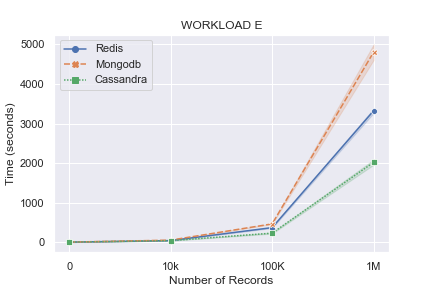
\includegraphics[scale =0.5] {images/performance/workloade}
            \label{performance.workloade}
            }
        \subfigure[Read-Insert-Update]{
            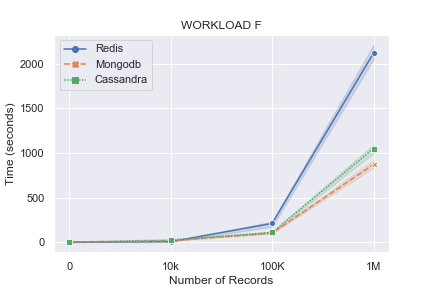
\includegraphics[scale =0.5] {images/performance/workloadf}
            \label{performance.workloadf}
            }
        \subfigure[Bulk Insert]{
            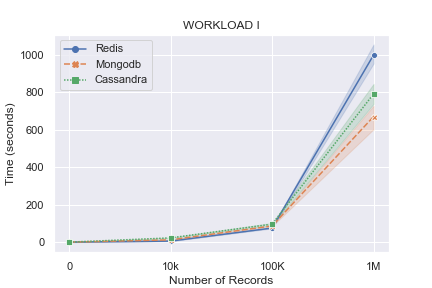
\includegraphics[scale =0.5] {images/performance/workloadi}
            \label{performance.workloadi}
            }
\end{figure}

\begin{figure*}[!h]
    \centering
    \label{performance.workloads.reads}
    \caption{Latencies of Workloads A to F and I – Latency of Read Database Operations for Different Number of Records}
        \subfigure[Read heavy]{
           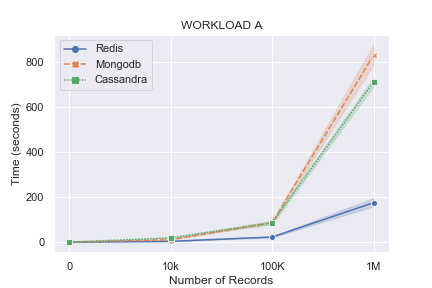
\includegraphics[scale =0.5] {images/performance/workloada}
           \label{performance.workloada}
         }
         \subfigure[Read mostly]{
           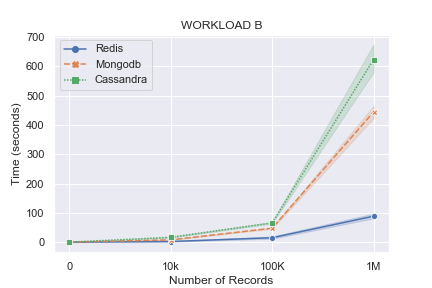
\includegraphics[scale =0.5] {images/performance/workloadb}
           \label{performance.workloadb}
         }
         \subfigure[Read only]{
           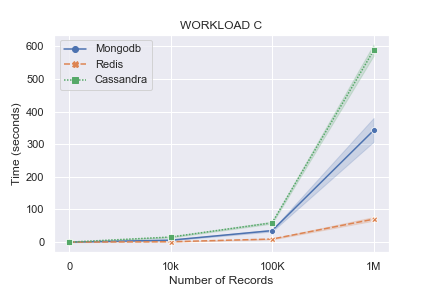
\includegraphics[scale =0.5] {images/performance/workloadc}
           \label{performance.workloadc}
         }
         \subfigure[Read latest]{
           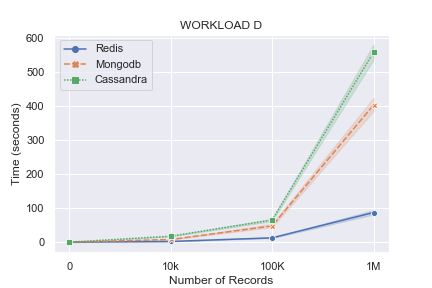
\includegraphics[scale =0.5] {images/performance/workloadd}
           \label{performance.workloadd}
         }
\end{figure*}



\subsection{Scalability}
% \ref{scalability.workloads}
Scalability is interpreted as the capacity of to   handle increasing load by having simultaneous and parallel task. 
The measurement focus of scalability in this study pertains to the maximum number of database operations in a single second (i.e. throughput) 
under increasing threaded processes or parallel loads.  Real-life application of threaded transactions can be seen during scenarios of multiple 
users using the system simultaneously. The results in table above was deployed using the configuration of 128 threads 
using the 1,000 records, which is an optmistic projection on biobanking system usage. 
Results showed that Redis still outperformed others in all database operations (i.e. Workload A to I).  
Also as shown in the table, Workload I or Bulk Insert operations was left blank from this criteria, because using simultaneous multiple bulk inserts 
encountered issues of duplicate ‘unique’ identifiers for MongoDB and Cassandra; hence, it was excluded from the results for all database.\newline

\begin{figure*}[!hpb]
    \centering
    \label{scalability.workloads}
    \caption{Latencies of Workloads A to F and I – Latency of Read Database Operations for Different Number of Records}
        \subfigure[Read only]{
            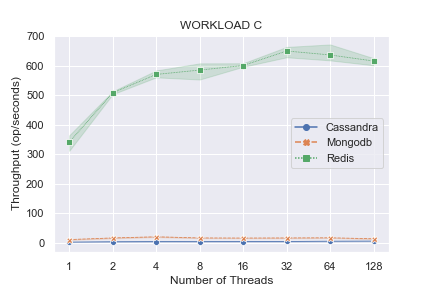
\includegraphics[scale =0.5] {images/scalability/workloadc}
            \label{scalability.workloadc}
        }
        \subfigure[Short Ranges]{
            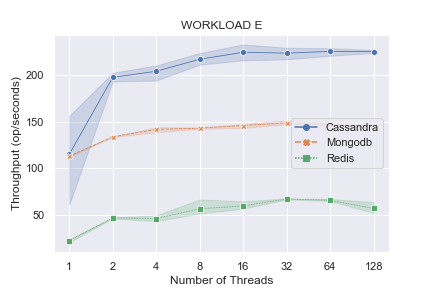
\includegraphics[scale =0.5] {images/scalability/workloade}
            \label{scalability.workloade}
        }
        \subfigure[Read-Insert-Update]{
            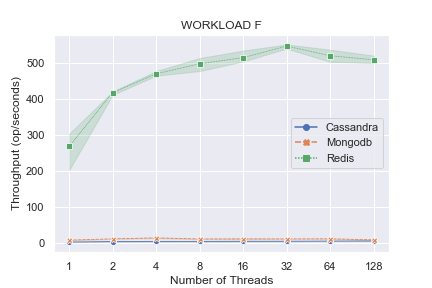
\includegraphics[scale =0.5] {images/scalability/workloadf}
            \label{scalability.workloadf}
        }
\end{figure*}

With the configuration of 128 threads on 1,000 patient records in a centralized or single node computing environment, 
it was found (as shown in Table 14.2) that there are significant differences in the scalability among the selected databases for all types of workload.
In addition, Table 14.1 revealed that Redis is significantly the most scalable for most of the workloads (except Workload F). 
On the contrary, the post analysis showed that Cassandra was the least scalable. 
This result supported the performance of Redis for 1,000 patient records shown in Figure 14.1; 
concisely, this experiment showed that Redis have the most efficient performance and scalability when subjected to smaller dataset (e.g. 1,000 patient records). 

\subsection{Storage} 
The table \ref{table.storage} shows the comparison of storage sizes when compared against the raw file, dataset sizes, and different databases. 
The four groupings of dataset were scaled by a factor of ten (10x); 
remarkably however, the storage size differences of in-between groupings had an average 90 percent more than the previous. 
For instance, the difference between first group (i.e. 1,000 records) to the next group (i.e. 10,000 records) is roughly 90 percent and the difference
for the succeeding group (i.e. 10,000 and 100,000 records) is also about 90 percent. 


\begin{table*}															
    \centering															
    \caption{Storage Sizes (GB) for FHIR Patient Resource}															
    \label{table.storage}															
    \begin{tabular}{llllllrc}   
        \toprule															
            NoSQL	&	NoSQL	&	\multicolumn{4}{c}{Number of Records}							&	Average size	&	Storage	\\
            Type	&	Database	&	1,000	&	10,000	&	100,000	&	1,000,000	&	per resource	&	Ratio	\\
        \hline	&		&		&		&		&		&		&		\\
            JSON files	&		&		&		&		&	 3.98 x 10-2	&	40.00 KB	&		\\
            Columnar	&	Cassandra	&	1.56 x 10-3	&	1.56 x 10-2	&	1.56 x 10-1	&	1.54	&	1.54 MB	&	+61.30\%	\\
            Document	&	MongoDB	&	3.46 x 10-3	&	3.45 x 10-2	&	3.45 x 10-1	&	3.45	&	3.45 MB	&	+25.12\%	\\
            Key-value	&	Redis	&	1.06 x 10-2	&	1.04 x 10-1	&	1.04	&	10.5	&	10.5 MB	&	-38.37\%	\\
        \hline
    \end{tabular}															
\end{table*}															

This indicates that the data storage storage scaling behavior of all three databases is strongly consistent. 
However, when the databases were compared to the average size of FHIR Patient resource in its raw JSON format, 
it was observed that the size changes by substantial degree. Among the three, Cassandra had the best storage rate of 61 percent 
decrease in size while the Redis had the most disk storage consumption with increase of 38 percent from the original file. 
However, these remarkable storage rate differences are by no means statistically significant when when subjected to inferential computation.

\subsection{Query Readability}
Four (4) scenarios were selected to represent different database operations: 
insert, update, search-aggregate, and multiple transactions. 
These query syntaxes are valid query language statements but in an abridged form. 
Meaning, not all database table variables and fields were shown in order to avoid technical intimidation among the study participants. 
The main goal of the query readability evaluation was to assessed the intuitiveness and ease of understanding 
of each database query structure and semantics. 
Though the results rely on the participants’ biases or lack thereof, it cannot be dismissed on grounds of subjectivity because measuring intuitiveness 
can also be targeted among participants with certain level or complete unfamiliarity to the particular subject of interest or topic. 
The participants’ responses were then subjected to inferential statistics and shown below.

\subsection{Flexibility}
Flexibility can be interpreted from many perspectives, among the common are technology architecture, deployment process, and schema capabilities. 
In this study, discussion of flexibility is taken from the latter perspective. 
By definition, it is defined as the capability to store dynamically changing data without having a predefined schema \cite{O.Schmitt20121,Z.Goli-Malekabadi201675}. 
However, flexibility is not totally equivalent to having no schema, but rather on the capacity to accommodate changes without substantial overhead requirements. 
Cassandra involves the need to write an additional parser in order to import and fit the raw nested JSON data into the columnar-wide type format that it currently supports.
For versions above 0.7, it was required to have columns and its data types be defined upfront \cite{J.Ellis2018}. From the initial approach of “schemaless”, 
it had transitioned into a “schema-optional”. Which meant, that it is heading back to where relational databases started: having predefined columns and data types. 
Thus, the original roadmap of being a schemaless approach was abandoned. This requirement is not necessary for native document-based databases like MongoDB among others. 
The raw data are simply imported using the original format of the dataset files; hence, full flexibility in data structure is experienced. 
In between is Redis, which requires minimal data transformation but is still considered schemaless. 
The data manipulation is need for the unique identifier of each item in a data in order for it to be segregated and stored separately as the key column,
the rest of the data is kept and bundled in the value column. To review, Cassandra is the the least flexible as it requires upfront pre-design of schema while MongoDB is most 
flexible as it can store any raw data in a flat or deeply nested JSON format.

\subsection{Extensibility}
Extensibility is capability to accommodate additional revisions on attributes, columns, and data types 
without the overhauling need to reconstruct or create new database \cite{S.Wang2013268}. 
Though, a lot of workarounds are available to model for extensibility and cover the inefficient schema design, 
at a certain point if the core infrastructure is inadequate, there is only so much patching that can be done before reaching the limits of the platform \cite{N.Ramachandran2016}.
Thus, a native, built-in, and inherent infrastructure is preferred to a “patch work” type of solution and temporary workaround.\newline

When comparing extensibility within NoSQL groups, no notable difference is observed since all the data structure can be extended either 
vertically (i.e. columnar-wide type) or horizontally (i.e. for both document-based and key-value types). 
Addition of new fields, columns and nested values are allowed without the need of much overhaul to existing schema for each approaches. 
However, it is noted that there is constraint of extensibility particularly to the Cassandra, as it requires additional 
“alter table” script in order for the new changes to be committed.


\section{Conclusion}
NoSQL database technology offers flexibility, extensibility, efficiency, and scalability where the traditional relational database fell short. 
This research adapted an evaluation framework for NoSQL databases and developed corresponding set of activities for its actual prototyping and testing. 
The study also described the execution of technical implementation set by the guidelines of the framework. With the foreknowledge that the type and 
the requirements of the application dramatically determine the appropriateness of database technology to use, the methodology highlighted the 
qualitative approach of eliciting the user requirements and the process of transforming into quantifiable evaluation criteria. 
Further, this paper aimed to make the methodology reproducible and the framework generalizable whilst adaptable to specific situations. 
Using the framework of evaluating data storage for healthcare domain, the study indicated that the NoSQL approach is a viable alternative to 
other traditional database design as it provides better query performance and scalability while still retaining certain degree of extensibility and flexibility. 
Among the shortlisted databases, MongoDB - a document type NoSQL was found to be the recommended choice for the current implementation and immediate need of the biobanking HIS.

\section*{Acknowledgements}

\subsection*{Funding} The biobank project “IHITM 2016-13: Establishment of a Philippine Cancer 
Phenome-Biobanking System and Biomonitoring Program” led by Prof. Michael C. Velarde (MCV) was funded by the Commission on Higher Education under
the Philippine-California Advanced Research Institute (PCARI) program. Also, the research itself was funded as stand-alone graduate funding under the same program. 

\subsection*{Author's Contributors} 
Approved the implementation: Dr. Maria Antonia E. Habana, Dr. Rodney B. Dofitas, 
Designed the workflow: Philip C. Sales (PCS). Performed the experiment: PCS, 
Programmed the scripts: PCS, Mycar Angelo B. Chu (MBC). Analyzed the results: PCS. 
Reviewed the paper: MCV, Dr. Alvin B. Marcelo (ABM), Prof. Ariel S. Betan (ASB), Prof. Bryann Chua, Dr. Jun Inciong. 
Wrote the paper: PCS, ABM, ASB, MCV.

\section*{Statement of Reproducibility}
To guarantee reproducibility of the results, all source codes, command scripts, configuration files, and Jupyter notes were deposited in a Github repository. 
All generated clinical datasets, benchmarking output files are also pre-generated and kept in same folder. 
In order to make the entire testing environment available for replication, server deployment configurations were packaged as container and is also publicly available in DockerHub link. 
Instructions written in the REAME.md was provided as quick-start guide for the actual implementation.

\section*{References}

\bibliography{mybibfile}




\end{document}